\chapter{System Architecture}\label{ch:architecture}
This chapter presents the architecture of the proposed reliable event processing system developed in \chref{ch:model}. The architecture defines the system’s structural organization, the responsibilities of its components, and the flow of events through the system under both normal operation and conditions involving missing observations.


\section{Architectural Overview}
\label{sec:architecture-overview}
At a high level, the system is organized around the processing of events originating from external sources. These events are propagated through an event stream, where their arrival is monitored to determine whether they should be forwarded directly for processing or reconstructed when expected observations are missing. Reconstructed events carry metadata that indicates the confidence of the underlying estimates, allowing this information to be taken into account during event processing. \figref{fig:domain-model} presents the domain model of the architecture, showing the key conceptual entities and their relationships.

\begin{figure}[t]
    \centering
    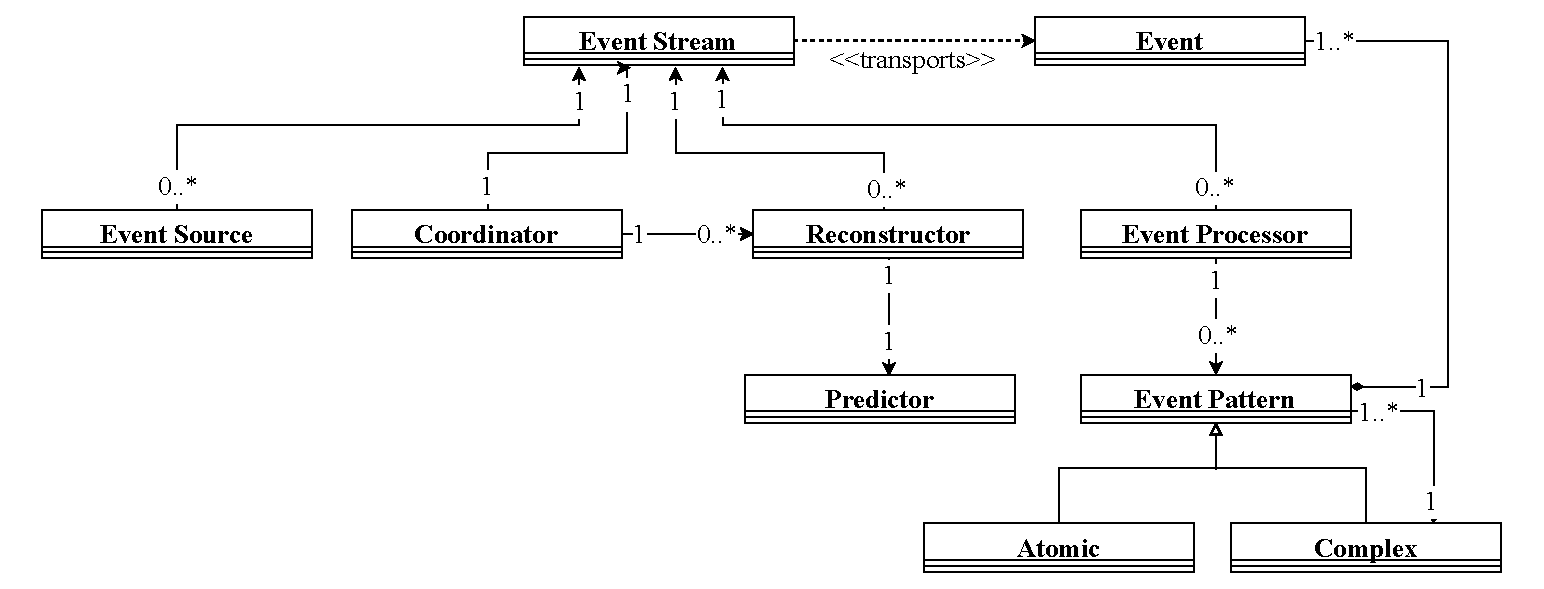
\includegraphics[width=\textwidth]{figures/Architecture/Domain Model.drawio.pdf}
    \caption{Domain model.}
    \label{fig:domain-model}
\end{figure}

An \emph{Event} represents an observation produced by an event source.  Events are propagated using an \emph{EventStream}, which provides a sequence of events to downstream elements of the system. \emph{Event sources} generate observations at specifc intervals but are assumed to be unreliable, allowing events to be absent.
To support reliable operation under such conditions, the architecture introduces explicit coordination and estimation elements. A \emph{Coordinator} monitors the arrival of events from each source and determines whether events arrive on time or are missing. When an expected event is absent from the \emph{EventStream}, a \emph{Reconstructor} uses a \emph{Predictor} to synthesize a replacement event. An \emph{Event Processor} consumes both observed and reconstructed events to evaluate event patterns.


\section{Component Architecture and Responsibilities}
\label{sec:architecture-components}

Figure~\ref{fig:component-model} presents the component model of the system, illustrating the major architectural elements and the interfaces through which they interact. The architecture separates concerns across event production, temporal coordination, state estimation, and event processing. All communication between components occurs through the \emph{EventStream}, which serves as the sole mechanism for propagating events through the system. This design enables components to interact through well-defined interfaces while remaining loosely coupled. The responsibilities of each component are described below.

\begin{figure}[t]
    \centering
    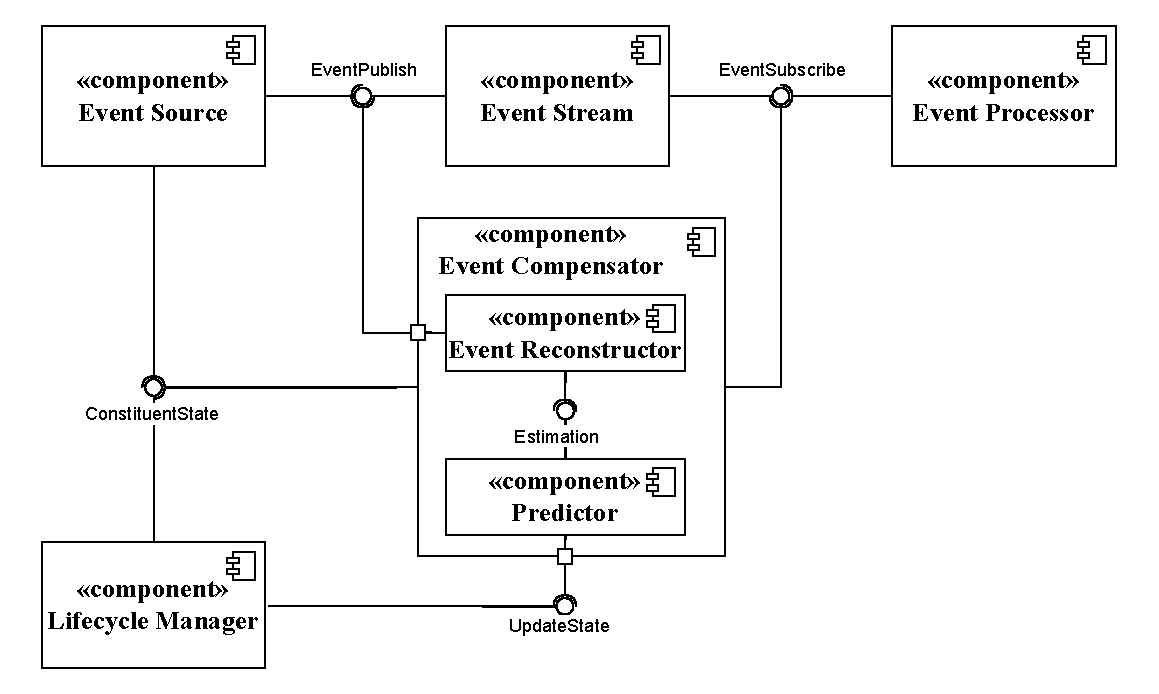
\includegraphics[width=\textwidth]{figures/Architecture/High Level Component Diagram.drawio.pdf}
    \caption{Component model.}
    \label{fig:component-model}
\end{figure}

\paragraph{Event Source}
An event source represents an external system, sensor, or data generator that produces observations of a monitored process. Its responsibility is to generate observations and encapsulate them as events that conform to the system’s event schema. These observed events are emitted into the event stream for downstream processing.

\paragraph{Event Stream}
The event stream provides a transport and routing abstraction for all events in the system. It acts as a shared event bus through which observed and reconstructed events are delivered to coordination, reconstruction, and processing components.

\paragraph{Coordinator}
The coordinator is responsible for monitoring the arrival of observed events and reasoning about their expected timing. For each event source, it maintains an expected schedule derived from configuration parameters such as reporting interval and tolerance. Based on this schedule, the coordinator identifies missing observations and initiates reconstruction when expected events do not arrive within the configured time window.

\paragraph{Reconstructor}
Each event source is associated with a reconstructor that manages reconstruction for that source. The reconstructor updates its internal state using observed events and performs reconstruction when notified of missing observations. For a missing event, it obtains an estimated value and associated confidence from its predictor, constructs a reconstructed event, and emits it into the event stream.

\paragraph{Predictor}
A predictor maintains an internal representation of the state associated with a specific event source. It supports state updates using observed values and state extrapolation to produce estimates when observations are missing. Predictors also provide uncertainty measures associated with their estimates, enabling confidence-aware processing.

\paragraph{Event Processor}
The event processor evaluates atomic and complex event patterns over the event stream. It consumes both observed and reconstructed events and applies pattern definitions to detect higher-level events. Confidence information associated with events may be incorporated into pattern evaluation to support uncertainty-aware detection.


\section{Event Processing and Reconstruction Flow}
\label{sec:architecture-sequence}

To illustrate the behaviour of the system, \figref{fig:sequence-model} presents the sequence model for event
processing and reconstruction.

\begin{figure}[t]
    \centering
    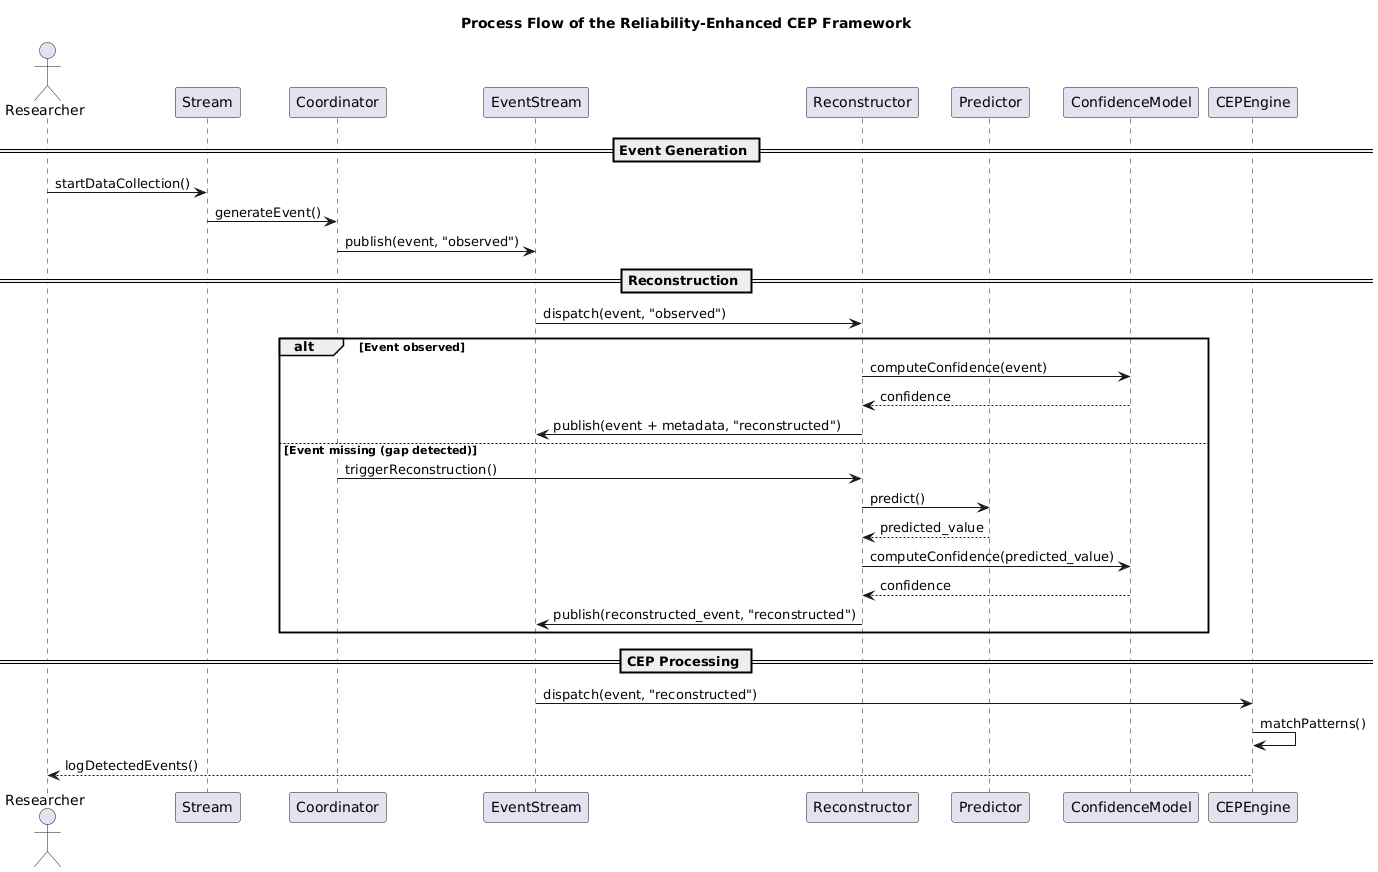
\includegraphics[width=\textwidth]{figures/Architecture/Sequence Diagram.png}
    \caption{Sequence model.}
    \label{fig:sequence-model}
\end{figure}

\paragraph{Normal Observation Flow}
When an observation is produced by an event source, it is encapsulated as an event and emitted to the event stream. The coordinator assesses whether the event arrives within its expected temporal window. If so, the event is consumed by the reconstructor, which forwards the observed value to its associated predictor for state update. In parallel, the event processor evaluates relevant event patterns over the event stream.

\paragraph{Missing Observation Flow}
If an expected event does not arrive within the expected time, the coordinator detects the absence and requests reconstruction. The reconstructor queries the predictor to obtain an estimated value and confidence for the expected time and emits a reconstructed event.



\section{Confidence-Aware Event Processing}
\label{sec:architecture-confidence-aware-cep}

The introduction of reconstructed events necessarily introduces uncertainty into the event stream. Rather than treating this uncertainty implicitly, the proposed architecture exposes it explicitly through confidence metadata, enabling event processing logic to take reconstruction reliability into account.

Confidence-aware event processing is achieved without modifying the core complex event processing (CEP) engine. Instead, confidence is represented as metadata associated with events and made available to queries through existing event access mechanisms. This design ensures that traditional event processing semantics are preserved while enabling additional reasoning when confidence information is present.

\subsection{Confidence Representation at the Event Level}

Confidence information associated with reconstructed events reflects the uncertainty of inferred values produced by the predictor. The architecture does not prescribe a specific confidence model; confidence may be represented as a scalar value, a vector of values, or a structured object, depending on the estimation technique and application requirements.

By representing confidence as metadata rather than as part of the core event payload, the architecture maintains backward compatibility with existing event consumers. Event processing logic that does not interpret confidence metadata continues to operate unchanged, while confidence-aware queries may selectively access this information.

\subsection{Mapping Confidence to Query Semantics}

At the query level, confidence information may be mapped to event processing semantics in different ways. For example, confidence may be used to filter events based on threshold criteria, to rank alternative event matches, or to weight event contributions in composite patterns. The architecture deliberately separates confidence representation from its interpretation, allowing different confidence handling strategies to be employed without modifying estimation or reconstruction components.

This separation supports flexibility in how confidence is used across different applications and processing contexts, and avoids coupling event processing logic to a particular estimation technique.

\subsection{Integration with CEP Engines}

The event processor interacts with the event stream using a conventional event-driven model, such as push-based or pull-based query evaluation, depending on the underlying CEP engine. Confidence metadata is accessed through query expressions when required, but the event processor does not assume any extensions to the CEP engine itself.

By confining confidence handling to query logic and metadata access, the architecture preserves compatibility with existing CEP engines. Confidence-aware event processing can therefore be introduced incrementally, alongside traditional event processing queries, without requiring changes to core CEP infrastructure.

